\section{Durchführung}
\label{sec:Durchführung}
In diesem Versuch werden Emissions- und Absorbtionsspektren verschiedener Stoffe untersucht.
Zum Vergleich der Güte der Messergebnisse müssen zunächst Literaturwerte recherchiert und berechnet werden. 
\subsection{Vorbereitungsaufgaben}
\label{subsec:vorbereitung}
Da das Emissionsspektrum von Kupfer untersucht werden soll, werden zunächst die hierfür nötigen Theoriewerte bestimmt.
Bei Kupfer liegt die $\symup{K}_\alpha$-Linie bei $\qty{8}{\kilo\electronvolt}$ \cite{NIST}. Daraus kann der zugehörige Bragg-Winkel $\Theta_{\symup{K}} = \qty{22.66}{\degree}$ 
ermittelt wereden. Die $\symup{Cu}\text{-}\symup{K}_{\beta}$-Linie liegt bei $\qty{8.95}{\kilo\electronvolt}$ mit einem Bragg-Winkel von $\Theta_{\symup{K}} = \qty{20.14}{\degree}$.

Für die fünf untersuchten Absorbermaterialien sind ebenfalls einige Literaturwerte von Relevanz, welche in \autoref{tab:vorbereitung} dargestellt sind.
\begin{table}
    \centering
    \caption{Literaturwerte für die Untesuchung der Absorbtionsspektren. $Z$ ist die Ordnungszahl des jeweiligen Elements, $E_K$ die Absorptionsenergie und $\sigma_K$
    die Abschirmkonstante. \cite{NIST}}
    \label{tab:vorbereitung}
    \begin{tabular}{l c S S S}
        \toprule
         & Z & {$E_{\symup{K}}^{\symup{Lit}} \mathbin{/} \unit{\kilo\electronvolt}$} & {$\Theta_{\symup{K}}^{\symup{Lit}} \mathbin{/} \unit{\degree}$} & {$\sigma_{\symup{K}}$} \\
        \midrule
        Zink         & 30 &  9.65 & 18.60 & 3.56 \\
        Gallium      & 31 & 10.37 & 17.29 & 3.61 \\
        Germanium    & 32 & 11.10 & 16.20 & 3.68 \\
        Brom         & 35 & 13.47 & 13.23 & 3.85 \\
        Rubidium     & 37 & 15.20 & 11.70 & 3.94 \\
        Strontium    & 38 & 16.10 & 11.04 & 4.00 \\
        Zirconium    & 40 & 17.99 &  9.86 & 4.10 \\
    \bottomrule
    \end{tabular}
\end{table}
\subsection{Versuchsaufbau}
\label{subsec:Versuchsaufbau}
Für diesen Versuch wird eine Kupfer-Röntgenröhre, ein LiF-Kristal, ein Geiger-Müller-Zählrohr und fünf Absorberproben verschiedener Elemente benötigt. 
Die Kupfer-Röntgenröhre, der LiF-Kristal und das Geiger-Müller-Zählrohr sind in einer geschlossenen Vorrichtung installiert, die über einen Computer gesteuert
werden kann. Diese ist in \autoref{fig:aufbau} zu sehen.

\begin{figure}
    \centering
    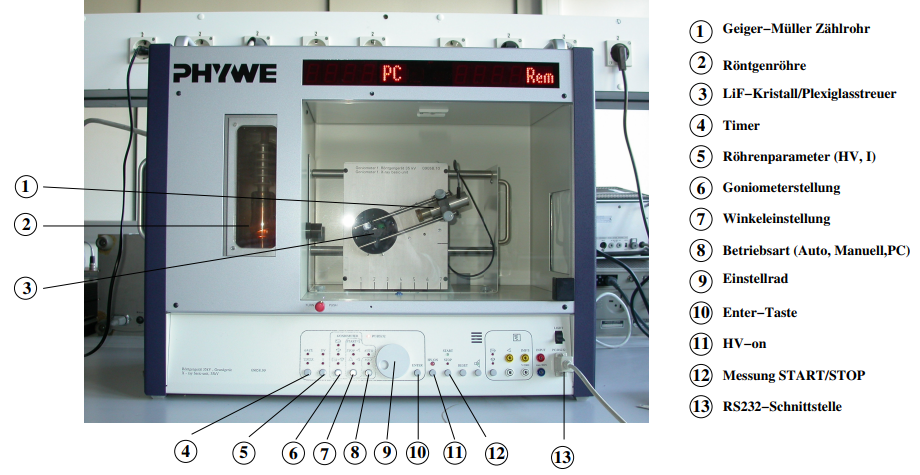
\includegraphics[width = \textwidth]{content/aufbauskizze.PNG}
    \caption{Aufbau der Kupfer-Röntgenröhre, des LiF-Kristals und des Geiger-Müller-Zählrohrs in einer Vorrichtung. \cite{v602}}
    \label{fig:aufbau}
\end{figure}

\subsection{Versuchsdurchführung}
\label{subsec:versuchsdurchführung}
Zu Beginn werden die Messapparatur und der Computer eingeschaltet. Auf dem Computer wird das Programm \textit{measure} gestartet.
Folgend wird in der oberen Leiste unter dem Menüpunkt \textit{Messgerät} das \textit{Röntgengerät} ausgewählt. Nun erscheint ein Einstellungsmenü.
Im ersten Teil des Versuches wird die Braggbedingung überprüft. Dazu muss die Neigung des LiF-Kristalls zu $\qty{14}{\degree}$ eingestellt werden. 
Im selben 
Menü wird für das Geiger-Müller-Zählrohr (im Folgenden \textit{GMZ} genannt) eine Winkelspanne von $\qty{26}{\degree}$ bis $\qty{30}{\degree}$ eingestellt. Der Winkelzuwachs
wird auf $\qty{0.1}{\degree}$ festgelegt. Die Integrationszeit sollte $\Delta t = \qty{5}{\second}$ betragen.
Nach Start der Messung werden Messwerte zu den angegebenen Winkeln genommen. Diese können in ein Textdokument gespeichert werden.

Es wird das globale Maximum der Messwerte ermittelt und mit dem Theoriewert, welcher aus der Braggbedingung berechnet werden kann, abgeglichen.
Bei Abweichungen von $\qty{1}{\degree}$ oder mehr sollten systematische Fehler ausgeschlossen und gegebenenfalls des Gerät neu kalibriert werden.

Anschließend wird das Emissionsspektrum der Kupferanode untersucht. Dazu wird zuerst in \textit{measure} der \textit{2:1 Koppelmodus} aktiviert. Für die erste Messung 
wird der Winkelbereich von $\qty{4}{\degree}$ bis $\qty{26}{\degree}$ eingestellt. Der Winkelzuwachs wird auf $\qty{0.2}{\degree}$ gestellt und die Integrationszeit bleibt 
unverändert. Es wird erneut die Intensität gemessen. Nach Vollendung der Messung lässt sich eine Grafik erstellen, welcher die $\symup{K}_\alpha$- und $\symup{K}_\beta$-Linien 
entnommen werden können. Anhand dieser Grafik wird nun ein möglichst kleiner Winkelbereich um die beiden Peaks gewählt. Mit diesem Winkelbereich und einem Winkelzuwachs von
$\qty{0.1}{\degree}$ wird erneut die Intensität gemessen, sodass ein Detailspektrum dargestellt werden kann
. 
Zuletzt werden die Absorptionsspektren verschiedener Stoffe untersucht. Dazu wird zuerst ein Zinkabsorber vor dem \textit{GMZ} befestigt.
Im Programm \textit{measure} wird ein Winkelzuwachs
von $\qty{0.1}{\degree}$ und eine Integrationszeit von $\Delta t = \qty{20}{\second}$ eingestellt. Da mit dieser Integrationszeit eine Messung über einen großen 
Winkelbereich sehr lange dauert, wird ein hinreichend großer, jedoch möglichst kleiner Winkelbereich gewählt. Dieser wird anhand \autoref{tab:vorbereitung} in einem Intervall
um den erwarteten Wert gewählt. Dieser Prozess wird für insgesamt fünf verschiedene Absorber wiederholt.
